\section{Qualitative results}
\label{sec:qual}

\Cref{fig:qual-monuseg,fig:qual-chaos} show predictions of the evaluated networks (EMA teachers with the reported weights). For MoNuSeg we show the test images with the largest, median and smallest per-image gain of CSSL over the recipe, and in each image the $256\times256$ window with the most annotated nucleus pixels. For CHAOS we show, in each split, the test slice with the largest annotated organ area. On the MoNuSeg image with the largest gain, the supervised model and the recipe mark large background regions as nuclei (per-image nuclei F1 33.9 and 41.3), while CSSL does not (79.0). On the median and smallest-gain images the predictions of the three models are close (CSSL and the recipe differ by at most 0.6 F1). On the CHAOS split 1 slice, CSSL recovers more of the liver and part of the spleen than the recipe (slice Dice 43.4 vs.\ 27.1); on splits 0 and 2 the predictions of all three models are close.

\begin{figure}[t]
  \centering
  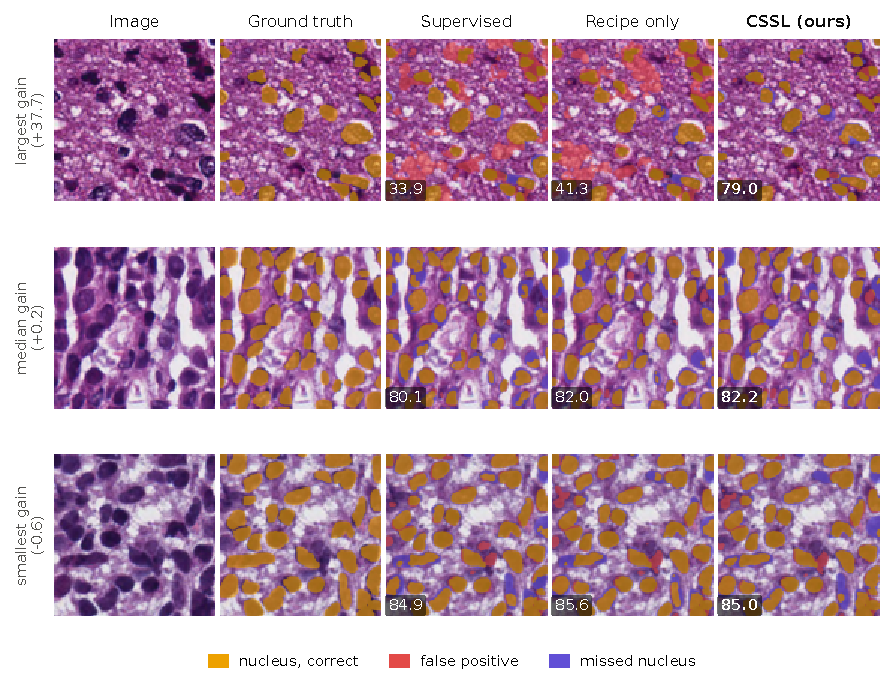
\includegraphics[width=0.98\linewidth]{figures/fig_qual_monuseg.pdf}
  \caption{\textbf{MoNuSeg test windows} (seed 0). Yellow: correctly segmented nucleus pixels. Red: false positives. Violet: missed nucleus pixels. Numbers are the nuclei F1 of the whole test image. Rows: the images with the largest, median and smallest gain of CSSL over the recipe (the gain in parentheses).}
  \label{fig:qual-monuseg}
\end{figure}

\begin{figure}[t]
  \centering
  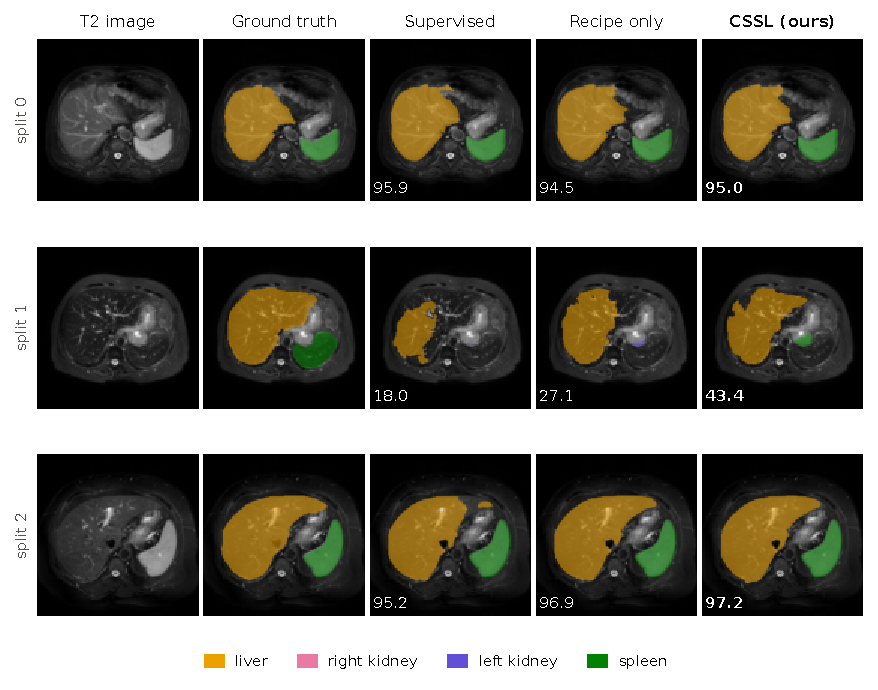
\includegraphics[width=0.98\linewidth]{figures/fig_qual_chaos.pdf}
  \caption{\textbf{CHAOS T2 test slices}, one per DAFNet split (the slice with the largest annotated organ area), best-validation checkpoints. Numbers are the mean organ Dice on the shown slice.}
  \label{fig:qual-chaos}
\end{figure}
